\documentclass[11pt]{article}
%\usepackage[14pt]{extsizes} % для того чтобы задать нестандартный 14-ый размер шрифта
%\usepackage[utf8]{inputenc}
\usepackage{mathtext}
\usepackage[english, russian]{babel}
\usepackage{amsmath}
\usepackage{amsfonts}
\usepackage{float}
\usepackage[margin=0.8in]{geometry}
\usepackage{multirow}
\usepackage{graphicx}
\usepackage[utf8x]{inputenc} % указать кодировку русского текста
\usepackage{fancyhdr}
\usepackage{indentfirst} % отступ в первой строке абзаца
\usepackage{wrapfig}
\usepackage{placeins}
\usepackage{wrapfig}
\usepackage{caption}
\usepackage{amssymb}
\usepackage{mathtools}
\usepackage[thinc]{esdiff}
\usepackage{cmap}
\usepackage[table,xcdraw]{xcolor}

\usepackage{breqn}

\pagestyle{fancy}
\begin{document}
\begin{titlepage}
\begin{center}
%\vspace*{1cm}
\large{\small ФЕДЕРАЛЬНОЕ ГОСУДАРСТВЕННОЕ АВТОНОМНОЕ ОБРАЗОВАТЕЛЬНОЕ\\ УЧРЕЖДЕНИЕ ВЫСШЕГО ОБРАЗОВАНИЯ\\ МОСКОВСКИЙ ФИЗИКО-ТЕХНИЧЕСКИЙ ИНСТИТУТ\\ (НАЦИОНАЛЬНЫЙ ИССЛЕДОВАТЕЛЬСКИЙ УНИВЕРСИТЕТ)\\ ФИЗТЕХ-ШКОЛА РАДИОТЕХНИКИ И КОМПЬЮТЕРНЫХ ТЕХНОЛОГИЙ}
\vfill
\line(1,0){430}\\[1mm]
\huge{Лабораторная работа 3.5.1}\\
\huge\textbf{Изучение плазмы газового разряда в неоне.}\\
\line(1,0){430}\\[1mm]
\vfill
\begin{flushright}
\normalsize{Устюжанина Мария}\\
\normalsize{\textbf{Группа Б01-107}}\\
\end{flushright}
\end{center}
\end{titlepage}
\fancyhead[L] {Работа 3.5.1}

\par \textbf{Цель работы:} изучение вольт-амперной характеристики тлеющего разряда; изучение свойств плазмы методом зондовых характеристик.
    
\par \textbf{В работе используются:} стеклянная газоразрядная трубка, наполненная неоном; высоковольтный источник питания; источник питания постоянного тока; делитель напряжения; потенциометр; амперметры; вольтметры; переключатели.

\section{Теоретическая часть и методика:}


 \textbf{Тлеющий разряд} -- электрический разряд в газе низекого давлнеия.
 
    \textbf{Свечение плазмы} -- следствие непрерывно идущей рекомбинации электронов и ионов в нейтральные атомы при относительно невысоких температурах. В этом процессе выделяется энергия и уменьшаеься концентрация электронов и ионов. В тлеющем газовом разряде обычно: <<горячие>> элктроны и <<холодные>> ионы: $T_e > > T_i$, так как масса электрона много меньше массы иона $m_e < < m_i$,следовательно, электроны ускоряются внешним полем почти без потерь энергии, а иону быстро отдают энергию от поля и электронов нейтральным атомам газа и стенкам сосуда.

\subsection*{Дебаевский радиус}

 Плазменные колебания могут быть возбуждены как за счёт внешнего воздействия (например, при прохождении электромагнитной волны), так и за счёт тепловой энергии, содержащейся непосредственно в плазме. Оценим амплитуду колебаний в последнем случае. Средняя скорость теплового движения электронов по порядку величины равна

\[ \bar{v_e} \sim \sqrt{\frac{K_{Б}T_e}{m_e}}\]


 где $T_e$ -- температура электронов. Амплитуду $r$ колебаний электронов относительно ионов оценим как смещение с тепловой скоростью $\bar{v_e}$ за характерное время плазменных колебаний $\frac{1}{w_p}: r = \frac{\bar{v_e}}{w_p}$. Зная, что $w_p = \sqrt{\frac{4\pin_e e^2}{m_e}}$, получим:
    
\[r_D = \sqrt{\frac{k_{Б}T_e}{4\pi n_e e^2}} \sim \frac{v_e}{w_p}\]

    Эту величину называют \textbf{дебаевским радиусом} (дебаевской длиной). Из рассмотренного примера видно, что дебаевская длина есть амплитуда ленгмюровских колебаний, возбуждаемых тепловыми флуктуациями. Она задаёт масштаб, на котором возможно спонтанное нарушение квазинейтральности плазмы.

    Таким образом, плазменная частота $w_p$ и дебаевская длина $r_D$ определят временную и пространственную масштабы коллективного движения электронов относительно ионов.


\subsection*{Плазменная частота}

\begin{figure}[H]
    \centering
    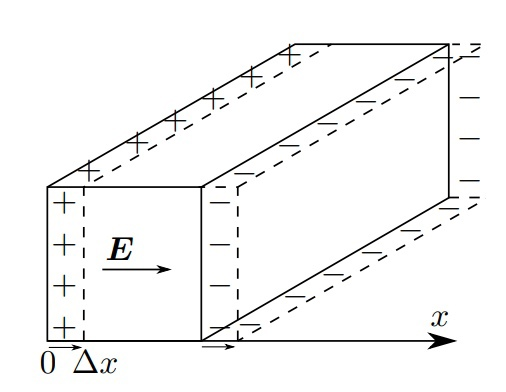
\includegraphics[width=0.3\textwidth]{plch_351.jpg}
    \caption{Плазменные колебания}
    \label{spec_1}
\end{figure}


    Теперь выделим параллелепипед с плотностью $n$ электронов, сместим их на $x$. Возникнут поверхностные заряды плотностью $\sigma = nex$, поле от которых $E = 4\pin_e \Delta x$ будет придавать электронам ускорение:

    
\[
\dfrac{d^2x}{dt^2}=-\dfrac{eE}{m}=-\dfrac{4\pi n e^2}{m}
\]

    откуда получаем уравнение гармонических колебаний:
    
\[\Ddot{\Delta x} + \frac{4 \pi n_e e^2}{m} \Delta x = 0 \]


    Следовательно, \textbf{плазменная (ленгмюровская) частота} колебаний электронов:
    
\begin{equation}
\omega_p = \sqrt{\dfrac{4\pi ne^2}{m}}.
\end{equation}

    Нами получен один из важнейших параметров плазмы. Плазменная частота определяет характрный временной масштаб плазы - время отклика на флуктуацию плотности заряда в ней. Часот аопределяет многие физические процессы, включая распространение электромагнитных волн в плазме.


\subsection*{Равновесная и неравновесная плазма}

    \textbf{Равновесная плазма} - плазма, в которой в состоянии теплового равновесия все частицы (электроны, ионы, нейтральные) имеют максвелловское распределение по скоростям, а их температуры равны: $T_e = T_i = T_n$.
    При тепловом равновесии с окружающей средой равновесная плазма может существовать неограниченно долго.


    \textbf{Неавновесная плазма} - плазма, в которой имеет место разделение температур компонентов, образующих её. При прекращении действия внешних источников неравновесная плазма исчезает в течение малых долей секунды ($\sim 10^{-5} - 10^{-4}$).


    В нашем эксперименте плазма является неравновесной.


\begin{figure}[H]
    \centering
    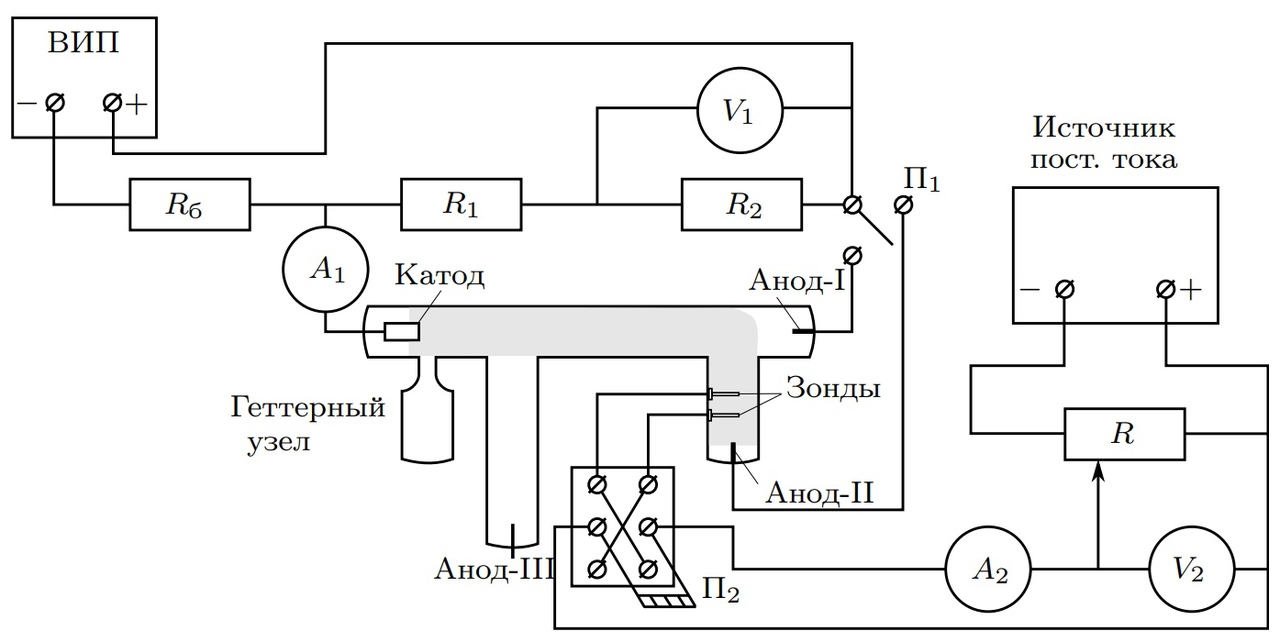
\includegraphics[width=0.8\textwidth]{sheme_351.jpg}
    \caption{Экспериментальная установка}
    \label{spec_1}
\end{figure}



\section{Ход работы:}

\subsection{Вольт-амперная характеристика разряда}
Установим переключатель \(\text{П}_1\) в положение "Анод-I". Установим напряжение, подаваемое с ВИП в 0.
Плавно увеличивая выходное напряжение ВИП, определим напряжение зажигания разряда \(V_{d}\) (По
показания вольиетра \(V_1\) непосредственно перед зажиганием). Получим: \(V_{d} = 230\; V\)

Снимем с помощью вольтметра \(V_1\) и амперметра \(A_1\) ВАХ разряда \(I_{d}\left(V_{d}\right)\). 
Изменять ток разряда \(I_{dsch}\) будем в диапазоне \(\left(0.5\; mA - 5\; mA\right)\). 

\begin{table}[H]
    \centering
    \begin{tabular}{|c|c|}
    \hline
    U, V  & I, mA \\\hline
    32    & 1.4   \\\hline
    31.9  & 1.8   \\\hline
    28.7  & 2.28  \\\hline
    27.8  & 2.8   \\\hline
    26.9  & 3.28  \\\hline
    25.7  & 3.8   \\\hline
    24.9  & 4.28  \\\hline
    24.4  & 4.8   \\\hline
    25    & 4.28  \\\hline
    25.6  & 3.8   \\\hline
    26.9  & 3.32  \\\hline
    27.6  & 2.8   \\\hline
    28.3  & 2.32  \\\hline
    31.96 & 1.8   \\\hline
    33.2  & 1.28  \\\hline
    34.3  & 0.8   \\\hline
    35    & 0.46  \\\hline
    \end{tabular}
\end{table}

\begin{figure}[H]
    \centering
    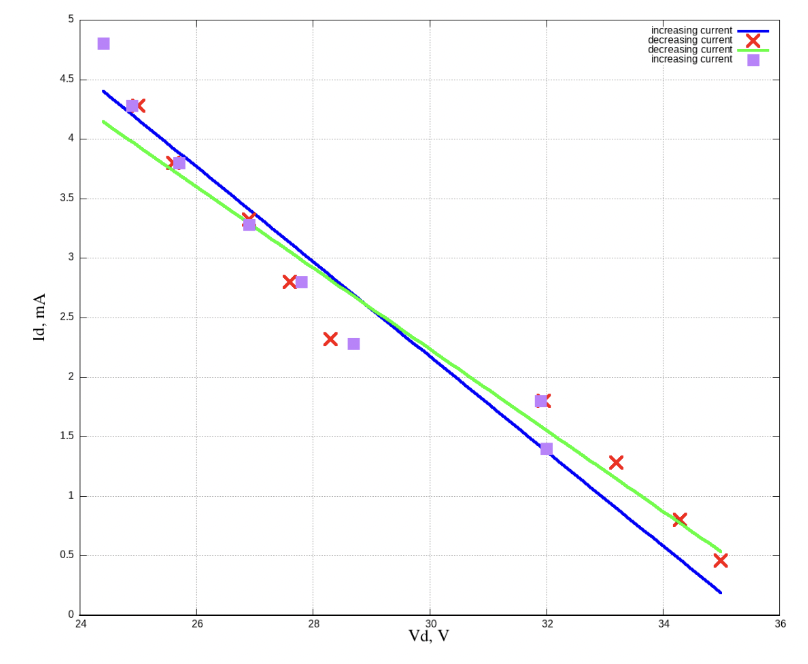
\includegraphics[width=0.5\textwidth]{V-A-1.png}
    \label{spec_1}
\end{figure}



Опроксимировав уравнением (\(y = kx + b\)) получим уравнения для уменьшения тока:
\[ k = (-0.34 \pm 0.02)\; mA/V \]
\[ b = (12.5 \pm 0.08)\; mA \]

И для повышения тока:
\[ k = (-0.40 \pm 0.03)\; mA/V \]
\[ b = (14.1 \pm 0.09)\; mA \]

Как видно из графиков, прямые очень похожи. По их наклону определим дифференциальное сопротивление разряда:
\[ R_{diff} = \frac{dV}{dI} = (-2.5 \pm 0.18)\cdot 10^{3}\: \Omega \]

\subsection{Зондовые характеристики}
Уменьшим напряжение ВИП до 0. Переведём переключатель \(\text{П}_1\) в положение "Анод-II",
переключатель \(\text{П}_2\) в положение "+".
Плавно увеличим напряжение ВИП и установим разрядный ток \(I_d = 5\:mA\). Включим в сеть источник
питания постоянного тока и установим на нем выходное напряжение \(V_2 = 25\:V\). При помощи
потенциометра \(R\) установим на зонде максимальное напряжение \(V_@ = 25\:V\).
С помощью амперметра \(A_2\) и вольметра \(V_2\) снимем ВАХ двойного зонда \(I_3\left(V_3\right)\).
Измерим ВАХ также при \(I_d = 3\: mA\) и \(I_d = 1.5\: mA\)

\begin{table}[H]
    \centering
    \begin{tabular}{|c|c|c|c|c|c|}
    \hline
    \multicolumn{2}{|c|}{\(I_d = 5\: mA\)}& \multicolumn{2}{|c|}{\(I_d = 3\: mA\)} & \multicolumn{2}{|c|}{\(I_d = 1.5\: mA\)} \\\hline
    \(V_3,\; V\) & \(I_3,\: mA\) & \(V_3,\; V\) & \(I_3,\: mA\) & \(V_3,\; V\) & \(I_3,\: mA\)\\\hline
    25 & 103  & 25          & 55& 25           & 27 \\\hline
    22 & 100  & 22          & 54& 22           & 26 \\\hline
    19 & 98   & 19          & 52& 19           & 25 \\\hline
    16 & 95   & 16          & 50& 16           & 24 \\\hline
    13 & 91   & 13          & 48& 13           & 23 \\\hline
    10 & 82   & 10          & 45& 10           & 21 \\\hline
    8  & 74   & 8           & 40& 8            & 19 \\\hline
    6  & 62   & 6           & 34& 6            & 16 \\\hline
    4  & 49   & 4           & 26& 4            & 12 \\\hline
    2  & 31   & 2           & 14& 2            & 6.5\\\hline
    0.6& 18   & 0.6         & 6 & 0.6          & 2  \\\hline
    -0.6 &17  & -0.6        & 4 & -0.6         & 2  \\\hline
    -2 & 29   & -2          & 13& -2           & 6  \\\hline
    -4 & 49   & -4          & 24& -4           & 12 \\\hline
    -6 & 63   & -6          & 34& -6           & 16 \\\hline
    -8 & 75   & -8          & 41& -8           & 19 \\\hline
    -10& 85   & -10         & 47& -10          & 22 \\\hline
    -13& 94   & -13         & 50& -13          & 24 \\\hline
    -16& 100  & -16         & 53& -16          & 25 \\\hline
    -19& 103  & -19         & 55& -19          & 26 \\\hline
    -22& 106  & -22         & 56& -22          & 27 \\\hline
    -25& 109  & -25         & 58& -25          & 28 \\\hline
    \end{tabular}
\end{table}

\subsubsection*{\(I_d = 5\: mA\):}


\begin{figure}[H]
    \centering
    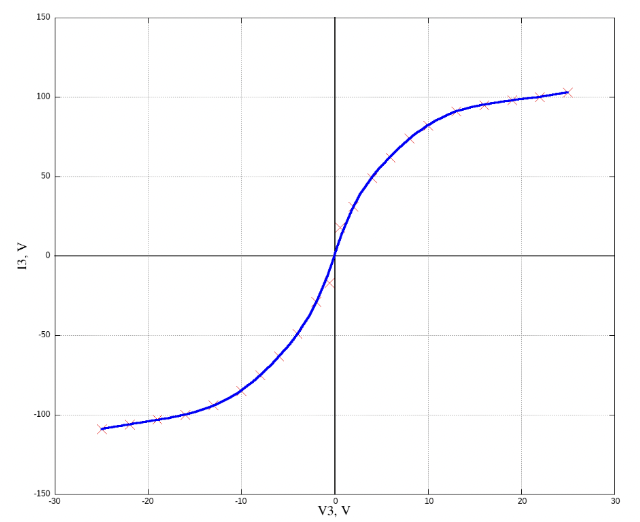
\includegraphics[width=0.5\textwidth]{V-A-5.png}
\end{figure}

\subsubsection*{\(I_d = 3\: mA\):}
\begin{figure}[H]
    \centering
    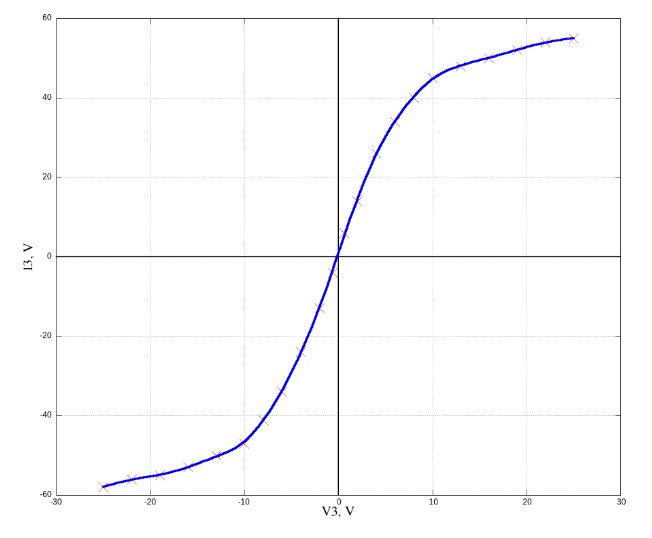
\includegraphics[width=0.5\textwidth]{V-A-3.png}
\end{figure}

\subsubsection*{\(I_d = 1.5\: mA\):}
\begin{figure}[H]
    \centering
    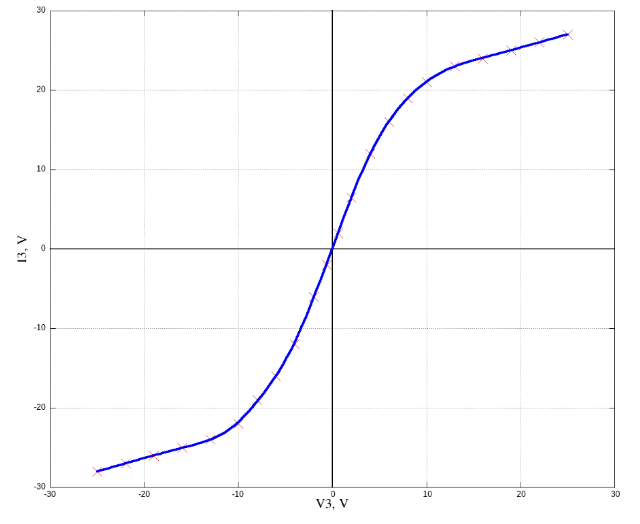
\includegraphics[width=0.5\textwidth]{V-A-1.5.png}
\end{figure}

По ВАХ для всех трёх значений \(I_d\) легко убедиться что участки кривой при больших напряжениях
выходят на асимптоты.

Из графиков вычислим температуры электронов \(T_e\).
Вычислим концентрацию электронов \(n_e\) по формуле
\[ I_s = 0.4n_eeS\sqrt{\frac{2kT_e}{m_i}} \]
Расчитаем плазменную частоту колебаний электронов по формуле
\[ \omega = \sqrt{\frac{4\pi n_e e^2}{m_e}} = 6\cdot 10^{-4} \sqrt{n_e}  \]



\begin{table}[H]
    \centering
    \begin{tabular}{|c|c|c|c|c|c|c|}
    \hline
    \(I_d,\; mA\)&\(T_e,\; 10^{4}K\) & \(n_e,\; 10^{18}m^{-3}\) & \(\omega,\; 10^{6}rad/sec\) & \(r_{D_e},\; cm\) & \(r_D,\; cm\) & \(N_D\) \\\hline
    5   &  3.14 & 4.9  & 1.3 &  0.5    &   0.05     &  256  \\\hline
    3   &  3.6  & 2.8  & 1.0 &  0.7    &   0.07     &  704  \\\hline
    1.5 &  3.6  & 1.4  & 0.7 &  1.0    &   0.095    &  1700 \\\hline
    \end{tabular}
\end{table}

Построим зависимости \(T_e(I_d)\) и \(n_e(I_d)\):

\begin{figure}[H]
    \centering
    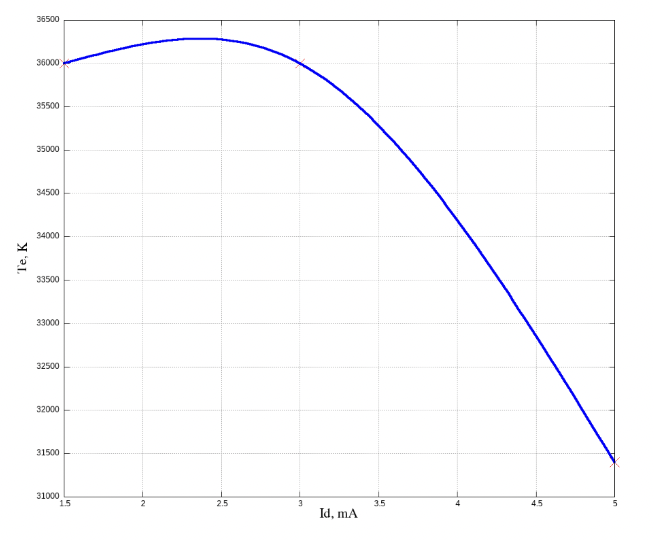
\includegraphics[width=0.5\textwidth]{T-I.png}
\end{figure}

\begin{figure}[H]
    \centering
    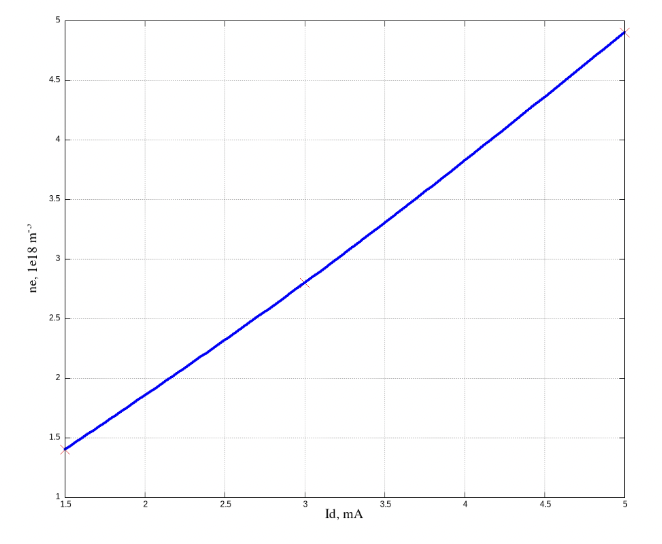
\includegraphics[width=0.5\textwidth]{n-I.png}
\end{figure}

\section{Выводы}

    В этой работе мы изучили ВАХ тлеющего разряда. Затем мы занялись изучением свойств плазмы методом зондовых характеристик. Мы получили что температура электронов у нас имеет пордок \(10^4\; K\), когда \(kT_e \simeq 1\; eV\). Концентрация электронов в плазме получилвсь порядка \(10^18\; m^{-3}\). Плазменная частота колебаний \(\omega \simeq 10^6 rad/sec\). Дебаевский радиус порядка \(10^{-3}\; m\) и число ионов в нём много больше единицы.


\end{document}